\section{GPU Profiling}

\frame{
	\frametitle{GPU Profiling}

	\begin{block}{What can be done}
		\begin{itemize}
			\item Gather GPU specific data
				\begin{itemize}
					\item[-] Hardware counters
					\item[-] Global GPU activity
				\end{itemize}

			\item Analyse and prove code improvements
		\end{itemize}
	\end{block}

	\begin{block}{What cannot be done}
		\begin{itemize}
			\item Compare CPU vs GPU implementations (except for global speedups)
			\item in-kernel profiling
		\end{itemize}

	\end{block}
}

\frame{
	\frametitle{GPU Profiling}

	\begin{block}{Limitations}
		\begin{itemize}%\itemsep=10pt
			\item Several Streaming Multiprocessors, but not all area measured
				% \begin{itemize}
					% \item Before Compute Capability 2.0, only 1 SM was measured
					% \item Later versions measure more than one (but still not all!)
				% \end{itemize}
			\item Harder to profile heterogeneous kernels

			\item Counters have different domains. Results may overlap

			\item Multi-context CUDA apps still lack support
		\end{itemize}

	\end{block}

	\begin{figure}
		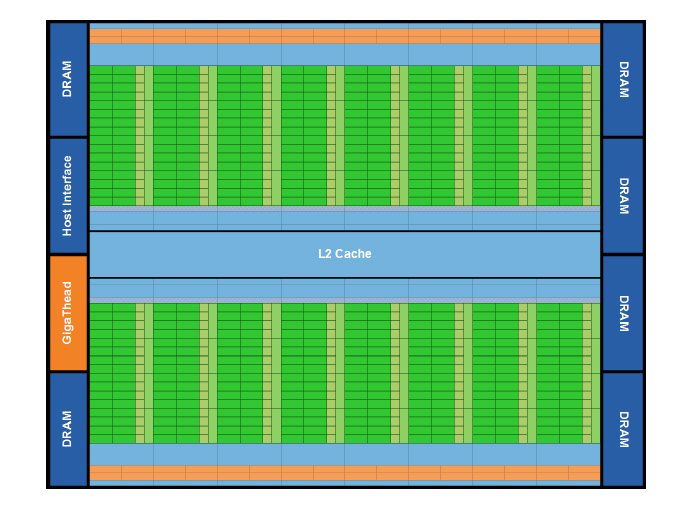
\includegraphics[height=.45\paperheight]{../images/fermi.jpeg}
	\end{figure}
}